\documentclass{beamer}
\usepackage{graphicx}
\usepackage{xcolor}

% Theme selection
\usetheme{Madrid}
\usecolortheme{default}

% Title parameters
\title{SWP OpenMP: Task 3 Kmeans}
\subtitle{Our CUDA Approach}
\author[F. Krückel, L. Hassel, G. Berner]{Group 1: Felix Krückel, Luke Hassel, Gerrik Berner}
\institute[RWTH]{RWTH Aachen}
\date{\today}


\usepackage{listings}
\usepackage{inconsolata}

\lstset{
  basicstyle=\ttfamily\footnotesize,
  columns=fullflexible,
  keepspaces=true,
  breaklines=true,
  breakatwhitespace=true,
  showstringspaces=false,
  frame=none,
  xleftmargin=0.3em,
  xrightmargin=0.3em,
  aboveskip=0.2em,
  belowskip=0.2em
}


%%%%%%%%%%%%%%%%%%%%%%%%%%%%%%%%%%%%%%%%%%%%%%%%%%%%%%%%%%%%%%%%%%%%%%%%%%%%%%%%%%%%%%%
\begin{document}

\frame{\titlepage}


%%%%%%%%%%%%%%%%%%%%%%%%%%%%%%%%%%%%%%%%%%%%%%%%%%%%%%%%%%%%%%%%%%%%%%%%%%%%%%%%%%%%%%%
\section{Recap: K-Means Algorithm}
\begin{frame}{Recap: K-Means Algorithm}

  \begin{enumerate}
    \item \textbf{Initialization:} Select $k$ initial centroids (randomly).
    \item \textbf{Assignment:} Assign each data point to the nearest centroid.
    \item \textbf{Update:} Recalculate centroids as the mean of assigned points.
    \item \textbf{Repeat:} Until convergence or max iterations.
  \end{enumerate}

  \vspace{0.4cm}
  \textbf{Pseudocode:}

  \begin{beamercolorbox}[rounded=true,shadow=true,sep=8pt]{block body}
    \ttfamily\small
    Initialize centroids = random(k)\\
    While not converged:\\
    \hspace*{1em}For point in data:\\
    \hspace*{2em}closest = argmin(distance(point, c))\\
    \hspace*{2em}assign(point, closest)\\
    \hspace*{1em}For c in centroids:\\
    \hspace*{2em}c = mean(assigned\_points)
  \end{beamercolorbox}

\end{frame}

\begin{frame}{Example}
  \centering
  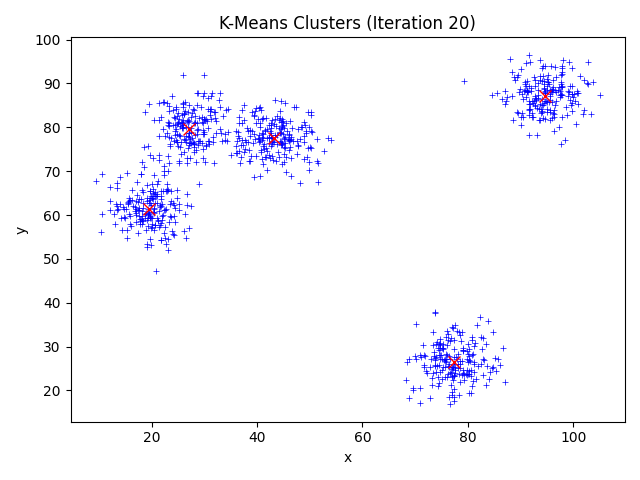
\includegraphics[width=0.7\textwidth]{clusters_final.png}

  Visualization of final cluster assignments.
\end{frame}

\begin{frame}{Computation Flow}
  \centering
  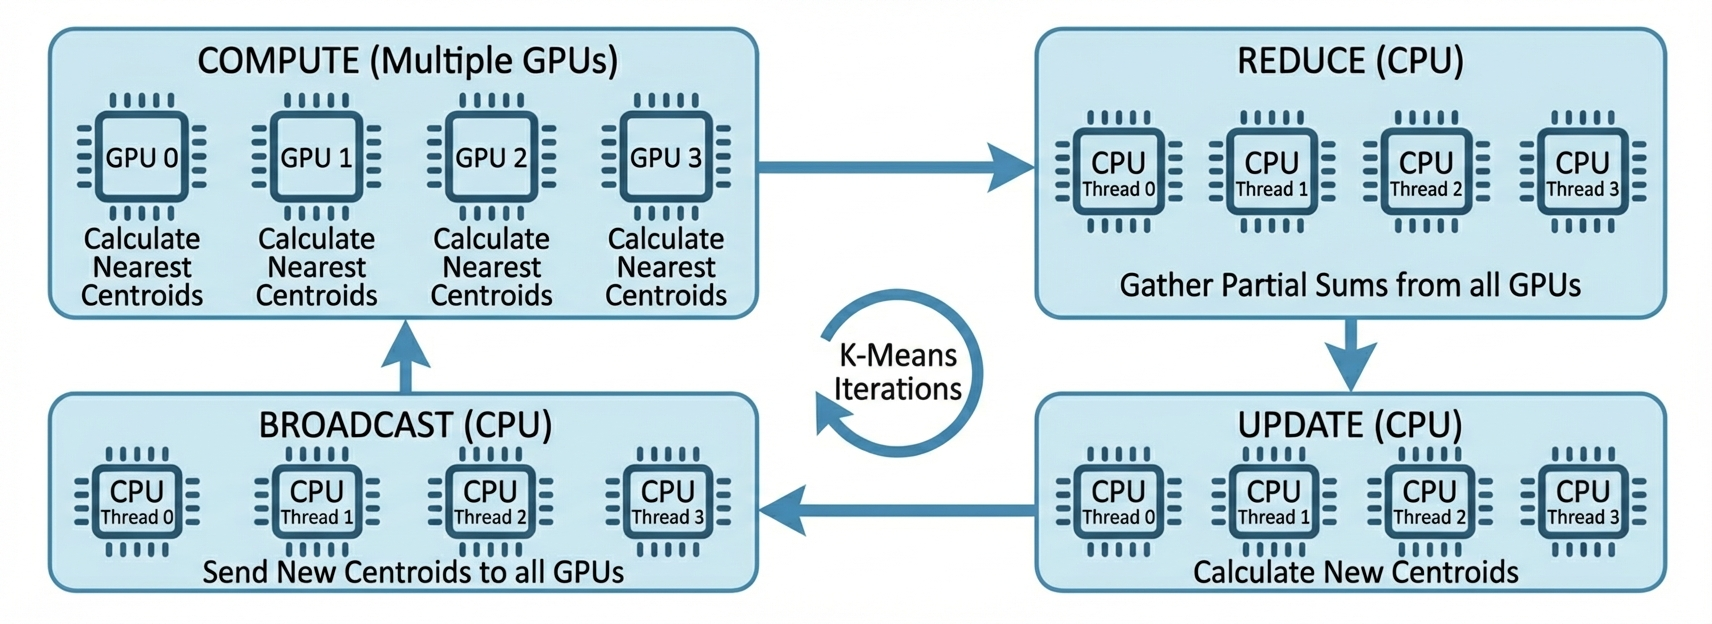
\includegraphics[width=0.9\textwidth]{images/flow.jpeg}

\end{frame}


\begin{frame}{Memory Utilisation}
  \centering
  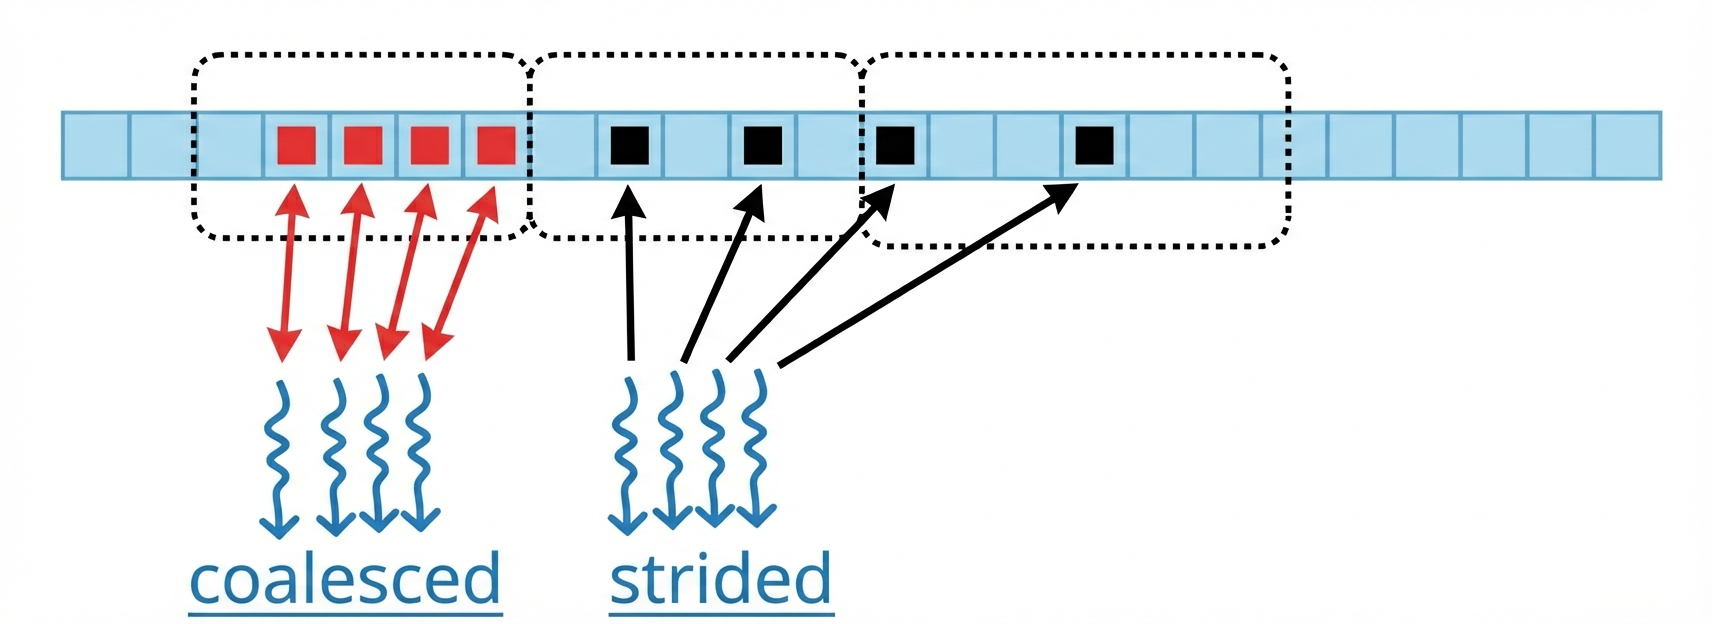
\includegraphics[width=0.5\textwidth]{images/coalesced.jpeg}

  Store the points and centroids in a coalesced manner:

  [x0, y0, x1, y1, x2, y2, ...] \quad $\rightarrow$ \quad [x0, x1, x2, ...] AND [y0, y1, y2, ...]


\end{frame}

\begin{frame}{Memory Utilisation}
  \centering
  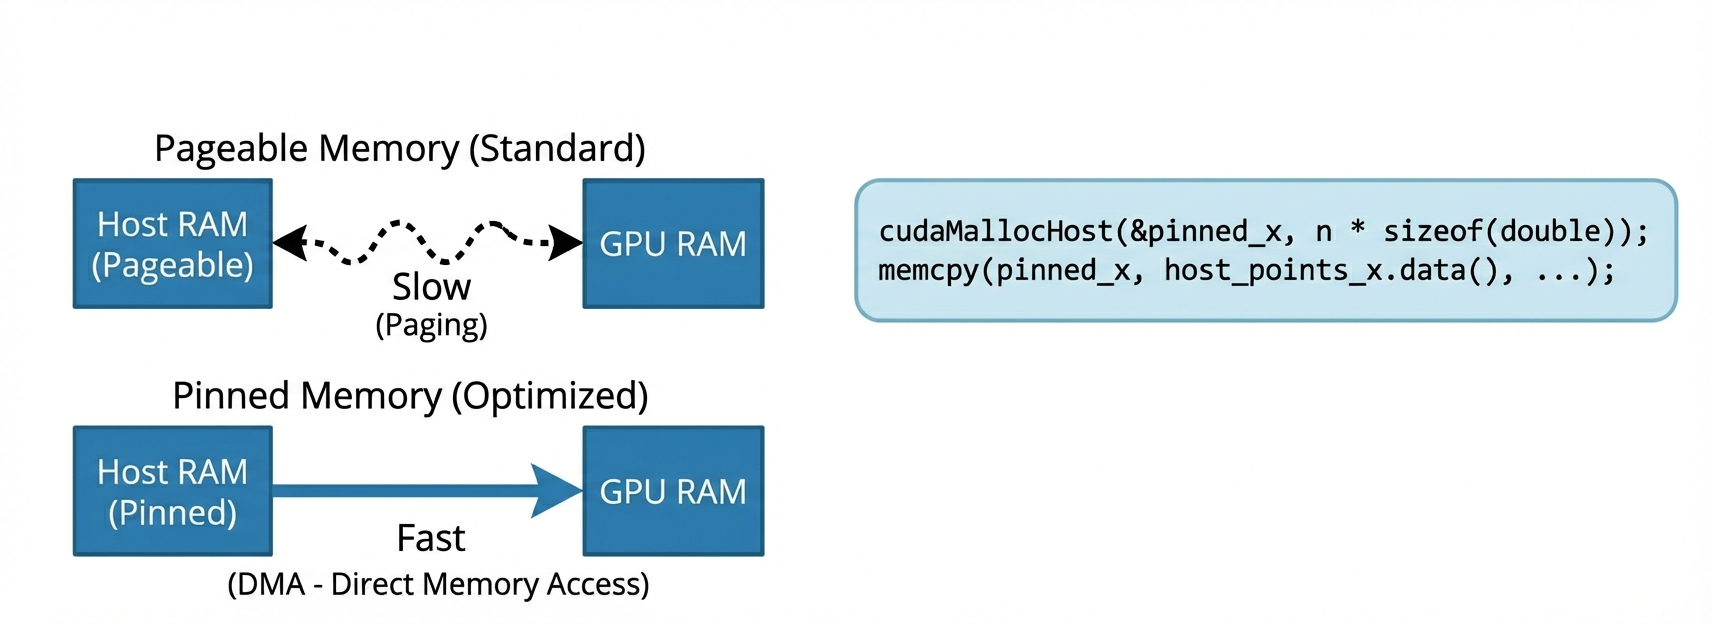
\includegraphics[width=0.8\textwidth]{images/pinned_memory.jpeg}

  \vspace{0.4cm}

  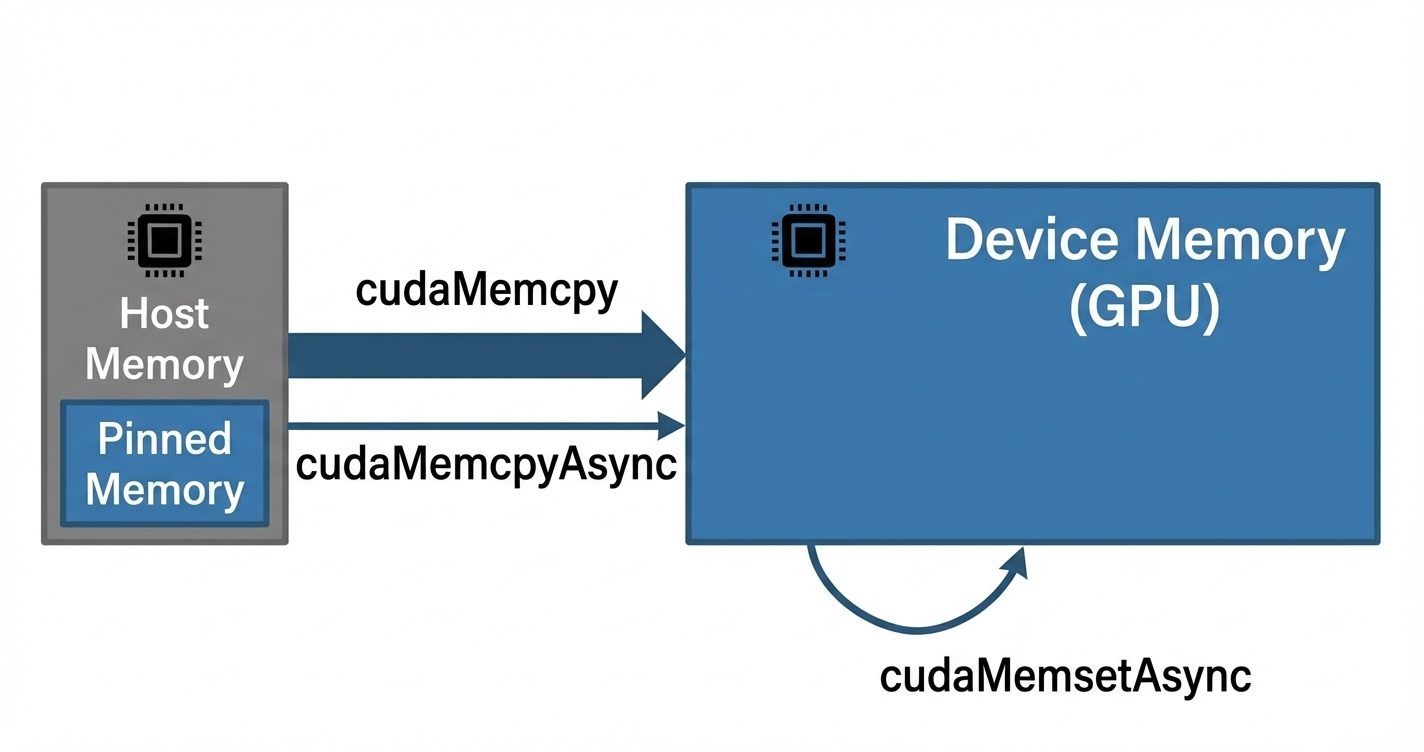
\includegraphics[width=0.5\textwidth]{images/allocation.jpeg}
\end{frame}


\begin{frame}{Memory Utilisation}
  \centering
  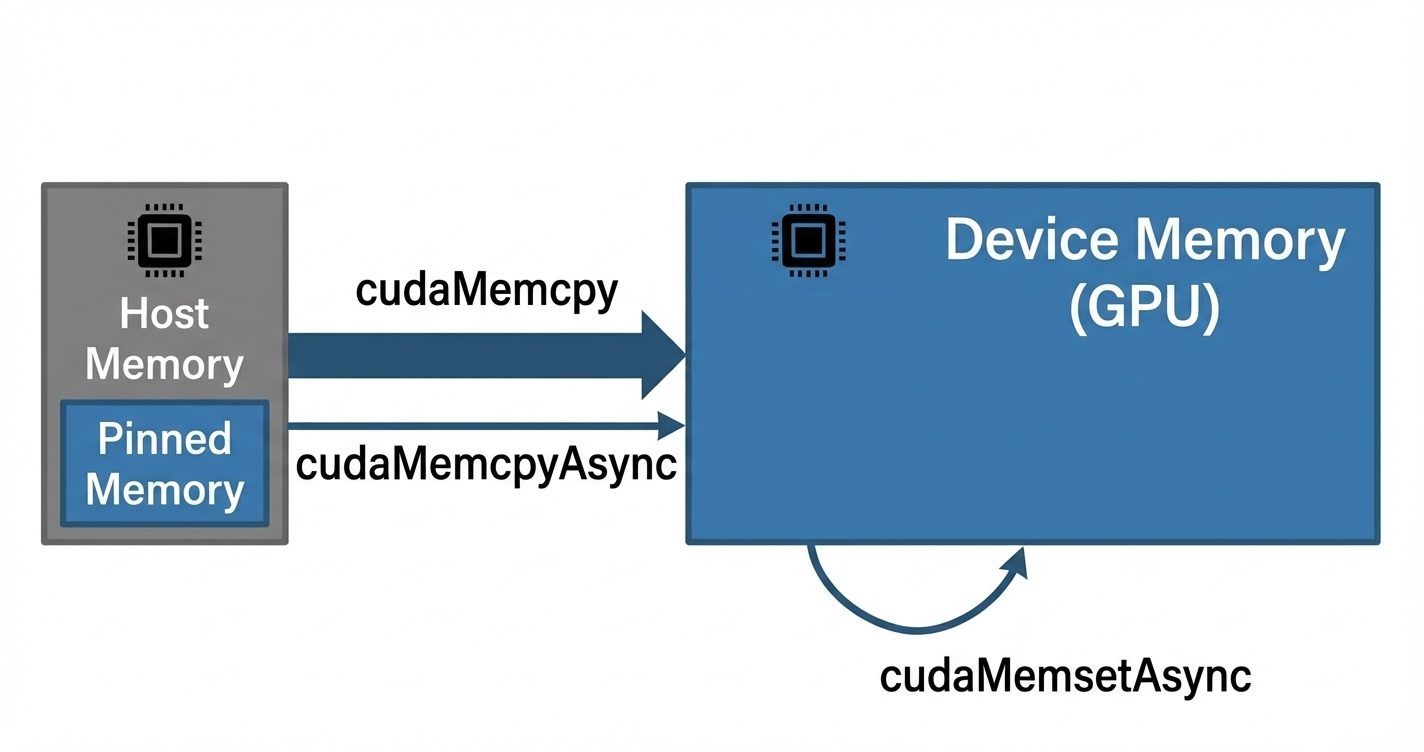
\includegraphics[width=0.5\textwidth]{images/allocation.jpeg}

  \vspace{0.2cm}
  \begin{itemize}
    \item \texttt{cudaMalloc(ptr, size)}: Allocates memory on GPU device
    \item \texttt{cudaMallocHost(ptr, size)}: Allocates \textbf{pinned memory} on host
    \item \texttt{cudaMemcpy(dst, src, size, dir)}: Synchronous copy between host $\leftrightarrow$ device
    \item \texttt{cudaMemsetAsync(ptr, val, count, stream)}: Asynchronously fills device memory with a constant byte value
  \end{itemize}
\end{frame}


\begin{frame}{Cache Blocking}
  \centering
  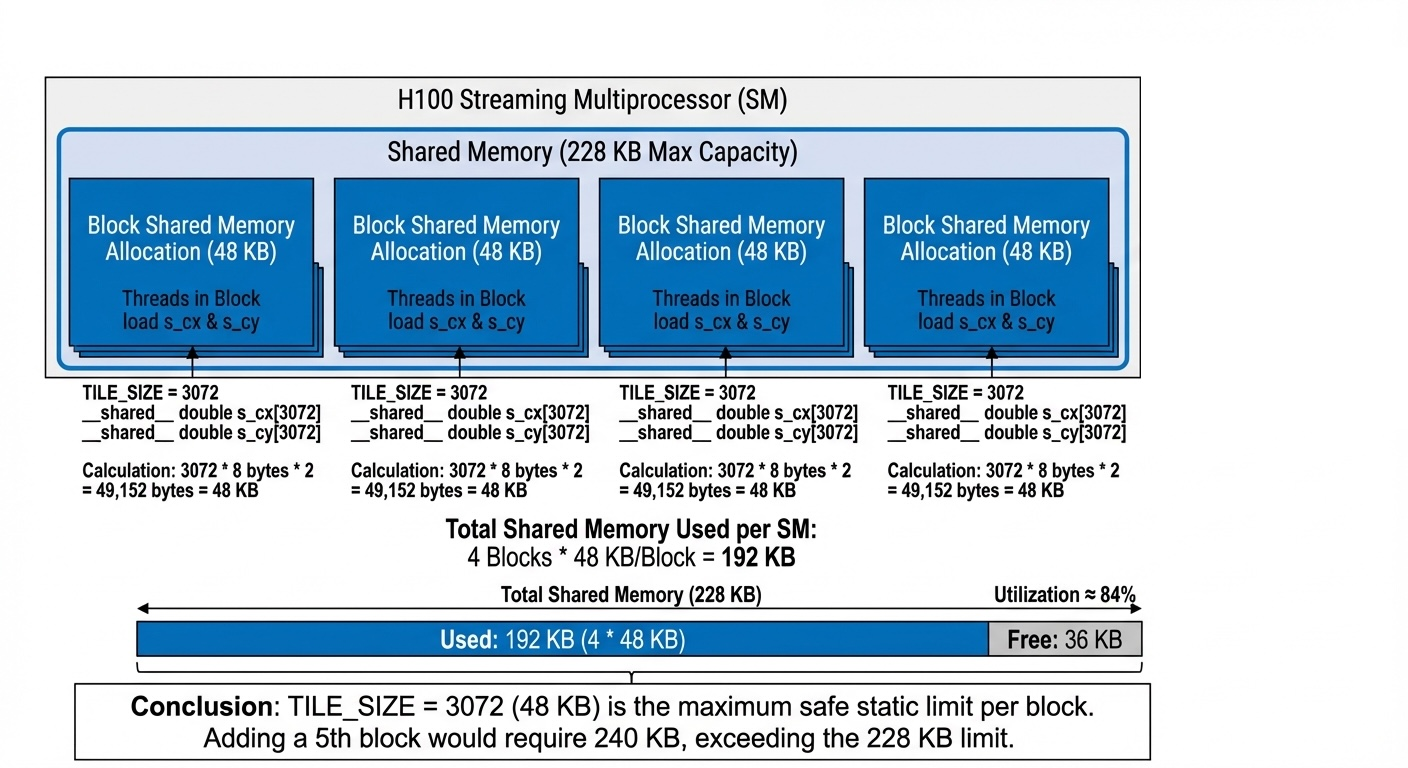
\includegraphics[width=1.1\textwidth]{images/shared_memory.jpeg}
\end{frame}


\begin{frame}{Performance Plots}
  \begin{columns}
    \begin{column}{0.5\textwidth}
      \centering
      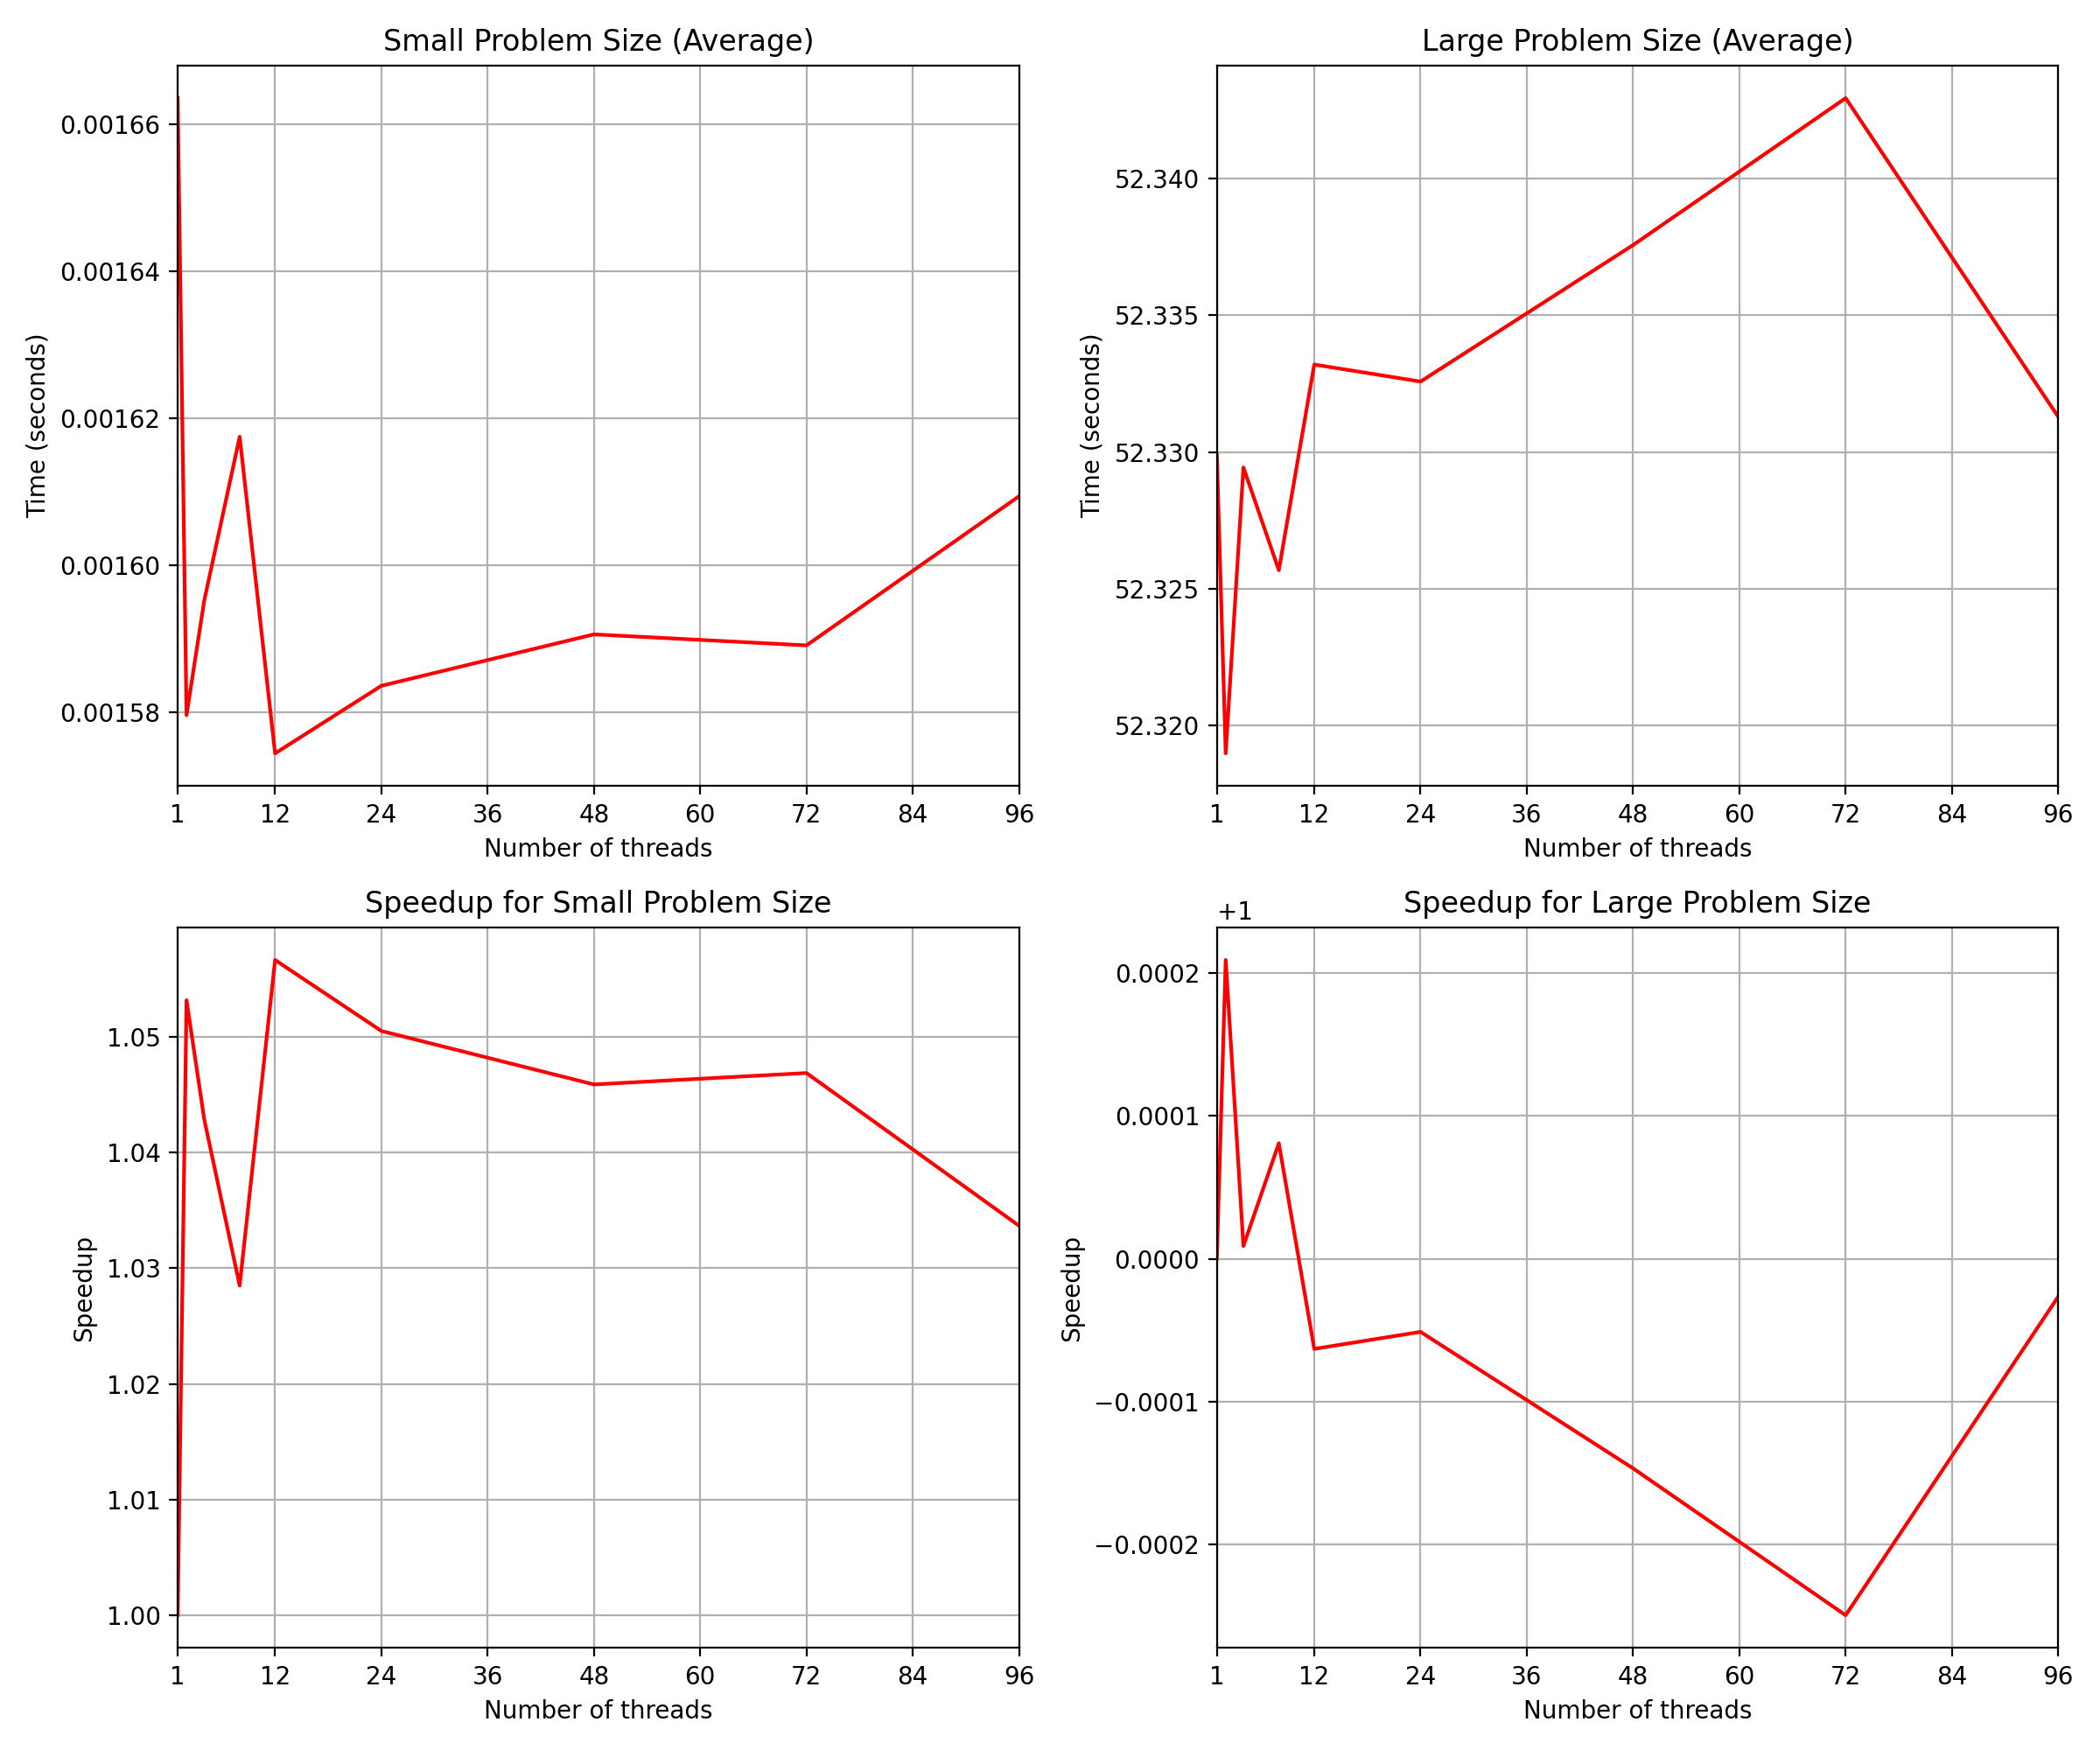
\includegraphics[width=\textwidth]{images/plot.png}
    \end{column}
  \end{columns}
\end{frame}


%%%%%%%%%%%%%%%%%%%%%%%%%%%%%%%%%%%%%%%%%%%%%%%%%%%%%%%%%%%%%%%%%%%%%%%%%%%%%%%%%%%%%%%
\newpage
\begin{frame}{Approximation}
  Instead of using the full dataset in every iteration, we use a random subset of it.


  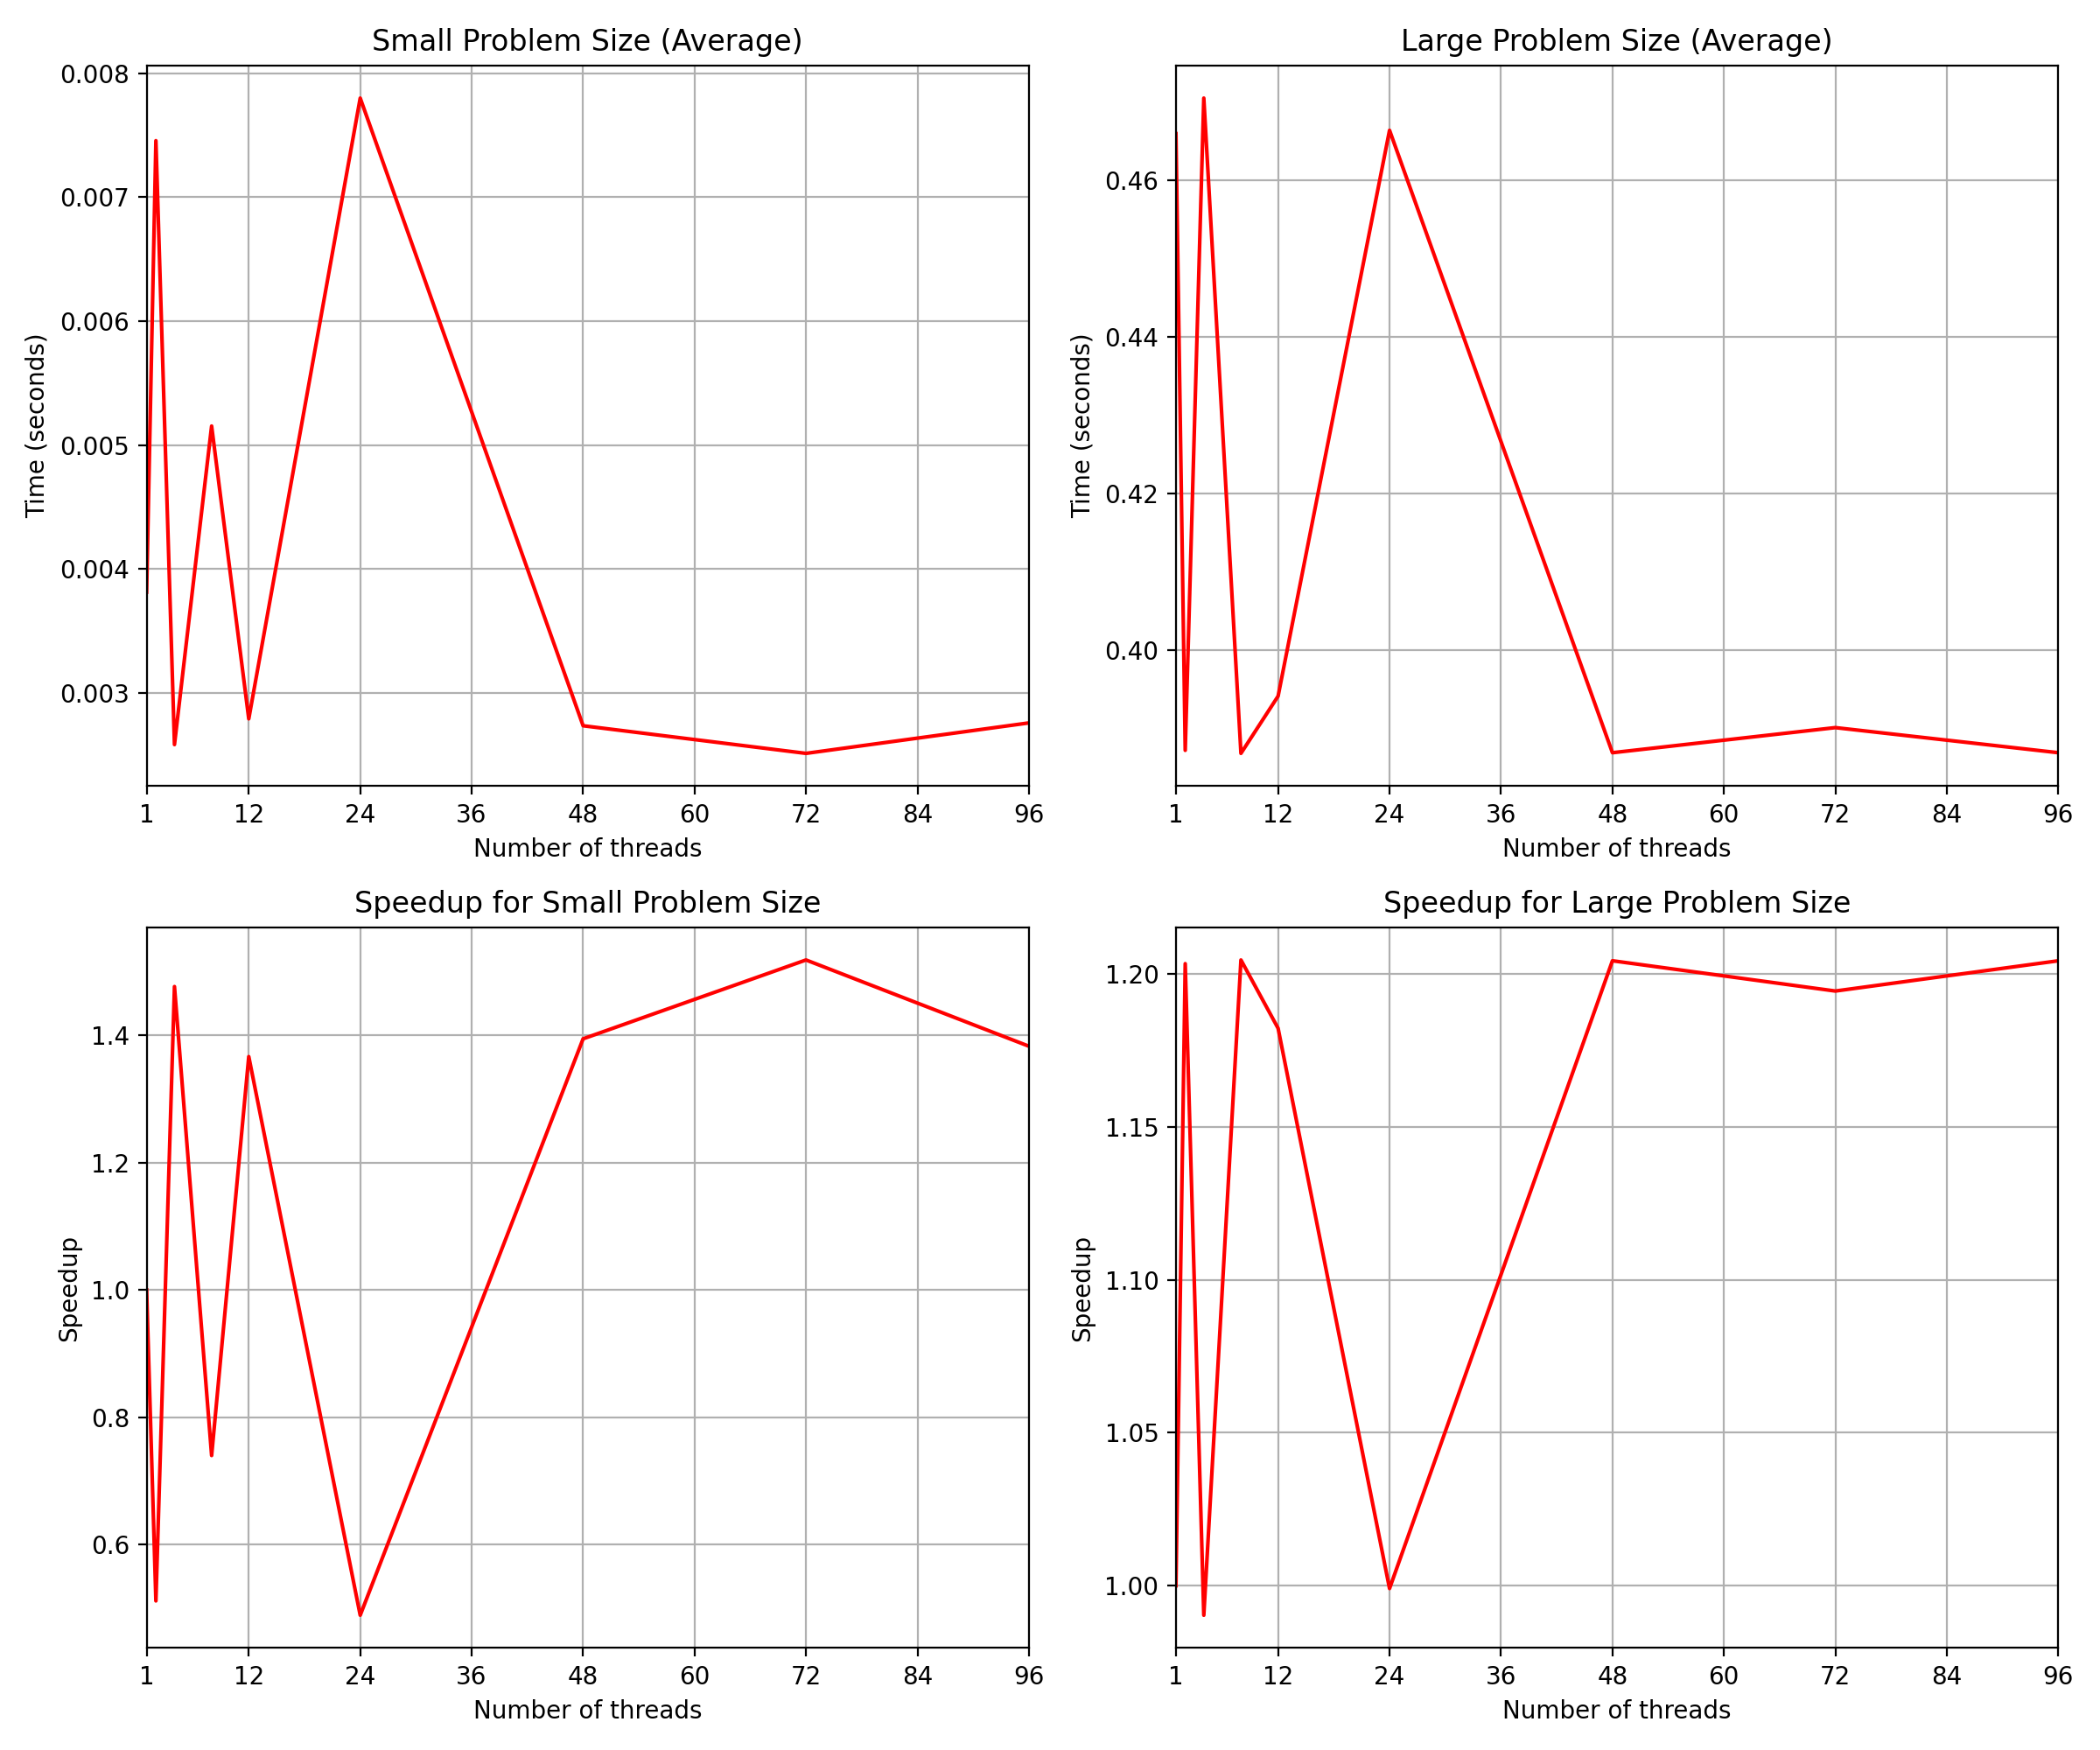
\includegraphics[width=0.5\textwidth]{plot_mini_batches.png}

\end{frame}

%%%%%%%%%%%%%%%%%%%%%%%%%%%%%%%%%%%%%%%%%%%%%%%%%%%%%%%%%%%%%%%%%%%%%%%%%%%%%%%%%%%%%%%



%%%%%%%%%%%%%%%%%%%%%%%%%%%%%%%%%%%%%%%%%%%%%%%%%%%%%%%%%%%%%%%%%%%%%%%%%%%%%%%%%%%%%%%

% \section{Future Work}
% \begin{frame}{Future Work}
%   \begin{itemize}
%     \item \textbf{GEMM Approach}:
%           \begin{itemize}
%             \item Reformulate distance calculation as Matrix Multiplication: $\|x - c\|^2 = x^2 + c^2 - 2xc$.
%             \item Leverage Tensor Cores on H100 for maximum throughput.
%             \item Potential for significant speedup over standard memory-bound kernels.
%           \end{itemize}
%   \end{itemize}
% \end{frame}



\end{document}
